\documentclass[12pt, openany]{book}
\usepackage{a4}
\usepackage{float}
\usepackage{graphicx}
\usepackage{amsmath}
\usepackage{amssymb}
\usepackage{epstopdf}
\usepackage{multirow}
\usepackage[procnames]{listings}
\usepackage{color}
\usepackage{tikz}
\usetikzlibrary{shapes, arrows}
\usepackage{physics}
\usepackage{xr}
\usepackage{amsfonts}
\usepackage{booktabs}
\usepackage{subcaption}
\usepackage[toc,page]{appendix}
\usepackage[nottoc,numbib]{tocbibind}
\usepackage{chemformula}
\usepackage{minted}
\usepackage{miller}
\usepackage{titlesec}
\usepackage{csquotes}
\usetikzlibrary{shapes.geometric, arrows}
% To get flow charts as eps
\usetikzlibrary{external}

\usepackage{wrapfig}  % text floating around figures
\usepackage{tabularx} % to control the width of tables and columns
\usepackage{setspace} % line spacing
\usepackage{fancyhdr} % line in Header

\usepackage[linktocpage, colorlinks, citecolor=black, linkcolor=black, urlcolor=black]{hyperref}  % having hyperlinks in black saves printing costs!

% Trying out new biblatex format
% Specifying how the references should be rendered
\usepackage[backend=bibtex8, style=phys, maxnames=12, articletitle=false, biblabel=brackets, chaptertitle=false, pageranges=false]{biblatex}

\hypersetup{pdftitle = {<title of your thesis>},
pdfauthor = {<your name>}, pdfkeywords = {<some>, <good>, <keywords>}}

\pagenumbering{arabic} %
\setlength{\parindent}{0.4cm}

\pagestyle{fancy}


%code mode
\definecolor{keywords}{RGB}{255,0,90}
\definecolor{comments}{RGB}{0,0,113}
\definecolor{red}{RGB}{160,0,0}
\definecolor{green}{RGB}{0,150,0}

\lstset{language=Python,
        basicstyle=\ttfamily\small,
        keywordstyle=\color{keywords},
        commentstyle=\color{comments},
        stringstyle=\color{red},
        showstringspaces=false,
        identifierstyle=\color{blue},
        rulecolor=\color{black},
        frame=single,
        tabsize=2,
        procnamekeys={def,class}}

% global change of font in tables
\newenvironment{tabschrift}{\begin{footnotesize}}{\end{footnotesize}}

\setlength{\evensidemargin}{0.0cm} %
\setlength{\oddsidemargin}{0.5cm} %
\setlength{\textwidth}{15.3cm} %
\setlength{\hoffset}{0cm} % = 1 inch + number

% Chapter in Header in lowercase
\renewcommand{\chaptermark}[1]{
\markboth{\chaptername \ \thechapter.\ #1}{}} %
\fancyhead{} \fancyhead[LE,RO]{\leftmark} %
\fancypagestyle{plain}{
   \fancyhf{}
   \fancyfoot[CE,CO]{\thepage}
   \renewcommand{\headrulewidth}{0pt}}
\fancyfoot{} \fancyfoot[CE,CO]{\thepage} %


\setlength{\headwidth}{\textwidth} % line in  header as wide as text

\setcounter{topnumber}{3}% default 2
\setcounter{bottomnumber}{3}% default 1
\setcounter{totalnumber}{6} % default 3


\renewcommand{\textfraction}{0.05} %default 0.2
\renewcommand{\topfraction}{0.95} % default 0.7
\renewcommand{\bottomfraction}{0.95} %default 0.3
\renewcommand{\floatpagefraction}{0.75} % default 0.5


% New command definitions to be used in the latex files
\newcommand{\kbT}{k_{\mathrm{B}} T}
\newcommand{\figpath}{figures}
\newcommand{\etal}{\textit{et al.}}
\newcommand{\abinitio}{\textit{ab initio}}


\DefineBibliographyStrings{english}{%
    andothers = {\em et\addabbrvspace al\adddot}
}
%adding the bibtex file name
\addbibresource{thesis.bib}

% Use this for adding a title page already rendere©d as pdf (with graphics as prescribed by your university)
\usepackage{pdfpages}
\begin{document}

\includepdf[pages=-]{chapters/title/title_page}

% Adding content like the abstract, toc, and so on.
\frontmatter
\chapter*{\centering Abstract}
\phantomsection
\addcontentsline{toc}{chapter}{Abstract}

This page contains the abstract which is usually about a page long (depending on the requirements set by your university) without any figures or tables.
\par
A reader should be able to understand the context of your work what you've acheived from reading this abstract alone.

\tableofcontents
\listoffigures
\listoftables

% The meat of your thesis, the different chapters
\mainmatter
% Creating chapters and subsections are demonstrated.

\chapter{Introduction}
\label{chap_intro}

These files contain the main text of your thesis. It's always a good idea to assign intuitive and unique labels for your chapters, sections and subsection since you can link to them at various places in your thesis. This sample chapter contains two sections: \ref{gen_intro} and \ref{specific_intro}. The first section has a subsection \ref{subsec_for_gen_intro}.

\section{General introduction}
\label{gen_intro}

Have some genreal introduction.

\subsection{Subsection of your general introduction}
\label{subsec_for_gen_intro}

A subsection in your general introduction.

\section{Specific introduction}
\label{specific_intro}

Some specific introduction to your topic.

\chapter{A chapter with equations, chemical formula, figures and tables}
\label{chap_main}

The previous chapter \ref{chap_intro} contained only some text. Here some sample
equations, chemical formula, figures, and tables
are introduced.

\section{Section with equations and chemical formula}
\label{sec_eq_fig_tab}

Materials science is highly interdisciplinary. So you will have to write complex
equations some condensed-matter physicists use like:

\begin{equation}
\expval{\hat{O}}{\Psi_e} = \int \dotsc \int \Psi_e^{*}(x_1,\dotsc,x_N) \hat{O}
\Psi_e(x_1,\dotsc ,x_N)  dx_1 \dotsi dx_N
\quad .
\label{main_eq1}
\end{equation}

and,

\begin{equation}
\braket{\Psi_e} = \int \dotsc \int |\Psi_e (x_1,\dotsc,x_N)|^2  dx_1\dotsi dx_N = 1
\quad .
\label{main_eq2}
\end{equation}

Sometimes, you would also have to write chemical formula like chemists:

\begin{equation}
\centering
\ch{H3O_{aq}+ + 2 H2O <-> H5O2_{(aq)}+ + H2O <-> H7O3_{(aq)}+} \quad .
\label{main_eq3}
\end{equation}

With the appropriate tex packages defined, all this is possible.

\section{Section with tables and figures}
\label{sec_tab_figs}

Here are some sample tables and figures. For the table, I've taken data from my
thesis and references \cite{Singh-miller2009, Sakong2018, Kittel1976, Salmeron1983}.

\begin{table}[!tbh]
\begin{center}
  \begin{tabular}{llc}
  \toprule
       &  a [\AA{}]  &  $\Phi\mathrm{_{Pt\hkl(111)}}$ [eV]  \\
  \midrule
  PBE (this work) &  3.97  &    5.69  \\
  PBE (ref. \cite{Singh-miller2009}) & 3.99  &    5.69   \\
  RPBE (this work) &  3.99 &   5.50 \\
  RPBE (ref. \cite{Sakong2018})&  3.99 &   5.51 \\
  Experiments &  3.92 \cite{Kittel1976} &   6.08 $\pm$ 0.15 \cite{Salmeron1983} \\
  \bottomrule
  \end{tabular}
\end{center}
\caption[Calculated lattice parameter of Pt and work function of the Pt\hkl(1 1 1)
surface.]{The calculated lattice parameter of bulk Pt and the work function of the
Pt\hkl(1 1 1) surface using different exchange-correlation functionals compared to
experimental values.}
\label{main_tab1}
\end{table}

\begin{figure}[!tbh]
\centering
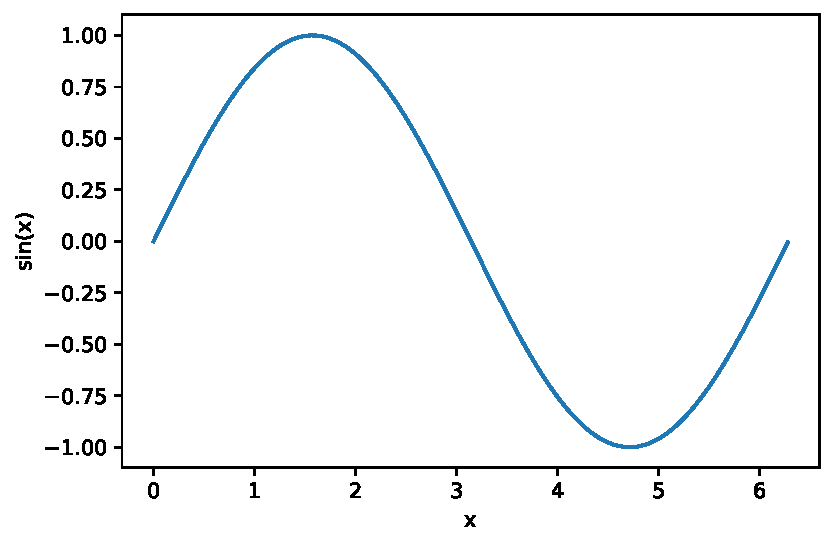
\includegraphics[scale=1., height=8cm]{\figpath/sinx.pdf}
\caption[A sinus curve]{A sinus curve to show how to include figures along with
captions.} %The text in square brackets is what is rendered in the list of figures.
\label{main_fig1}
\end{figure}

Notice how in table \ref{main_tab1}, I've rendered crystallographic directions using
the "miller" tex package.

\section{Section with code}
\label{sec_code}

If you are in a computational field, you might need to include some code in your
thesis. The "minted" TeX package is useful for this. For example, some python code
can be inserted the following way:

\begin{minted}{python}
    import numpy as np
    import matplotlib.pylab as plt
\end{minted}

You could also insert inline code like so: \mintinline{python}{numpy}.

\begin{appendices}
\label{appendix}
\chapter{Appendix chapter one}
\label{chap_app_1}

You could add the appendices in this file. The chapter labels work appropriately
(\ref{chap_app_1}). 


%Bibliography and stuff after your main text (Acknowledgements, CV, publications, etc.)
\backmatter
\chapter*{Bibliography}
\addcontentsline{toc}{chapter}{Bibliography}
\markboth{Bibliography}{Bibliography}
\printbibliography[heading=none]
%Stuff to be included after the bibliography
% These lines are necessary to adjust the spacing of the heading
\titleformat{\chapter}[hang]{\huge\bfseries}{\thechapter}{1em}{}
\titlespacing{\chapter}{0pt}{0pt}{1cm}

\chapter{Acknowledgments}

Thank your professors, colleagues, funding agencies, friends, and family. Usually,
people sign out by specifying the date and time of writing this thesis.
\\\\
D\"usseldorf, \today

\end{document}
